\documentclass{article}
\usepackage[portuguese]{babel}
\usepackage[dvipsnames,table,xcdraw]{xcolor}
\usepackage{amsthm,amssymb,mathtools}
\usepackage{ragged2e}
\usepackage[a4paper,top=1.5cm,bottom=2cm,left=2cm,right=2cm]{geometry}
\usepackage{setspace} \onehalfspacing
\usepackage{lastpage}
\usepackage{amsmath,amsthm,amssymb}
\usepackage{breqn}
\usepackage{amsmath,mathtools}
\usepackage[toc,page]{appendix}
\usepackage{tikz-cd}
\usepackage{environ}
\usepackage{subfigure}
\usepackage{tikz}
\usepackage[colorlinks=true, linkcolor=Blue, citecolor=Chocolate,linktocpage=true]{hyperref}

\tikzset{>=stealth}
\usetikzlibrary{calc,patterns,angles,quotes}
\usetikzlibrary{arrows}
\usepackage{tkz-euclide}
\usetikzlibrary{decorations.pathreplacing}
\newcommand{\colvec}[2][.8]{%
  \scalebox{#1}{%
    \renewcommand{\arraystretch}{.8}%
    $\begin{pmatrix}#2\end{pmatrix}$%
  }
}

%Definições dos ambientes do tipo teorema
\theoremstyle{plain}
\newtheorem{theorem}{Teorema}
\newtheorem{proposition}{Proposi\c{c}\~ao}
\newtheorem{corollary}{Corol\'ario}
\newtheorem{lemma}{Lema}
\newtheorem{observation}{Observa\c{c}\~ao}

%Definição dos ambientes do tipo definição
\theoremstyle{definition}
\newtheorem{definition}{Defini\c{c}\~ao}
\newtheorem{example}{Exemplo}

%Definição dos ambientes tipo observação
\theoremstyle{remark}
\newtheorem{remark}{Observa\c{c}\~ao}
\DeclareMathOperator{\rank}{rank}
\DeclareMathOperator{\vol}{vol}
\DeclareMathOperator{\ind}{ind}
\DeclareMathOperator{\mdc}{mdc}
\DeclareMathOperator{\de}{d}
\DeclareMathOperator{\be}{b}
\DeclareMathOperator{\spand}{span}
\DeclareMathOperator{\medi}{med}
\DeclareMathOperator{\modu}{mod}
\let\oldemptyset\emptyset
\let\emptyset\varnothing
\DeclarePairedDelimiterX{\inp}[2]{\langle}{\rangle}{#1, #2}
\DeclareMathOperator{\inter}{int}

\title{Códigos perfeitos em Reticulados Ambientes}
\author{Lucas Eduardo Nogueira Gonçalves, lucasedng@gmail.com}
\date{São José dos Campos - SP, Brasil}

\begin{document}
\maketitle

\section{Resultados}

\begin{theorem}\label{cods1}
  Seja $r>0$ um número natural de modo que $r \equiv 0\;(\modu\;2)$. Temos que o reticulado $\Lambda'$, com base $\beta' = \{(0,2(r+1)),(r+1,r+1)\}$ é um $r$-código linear perfeito em $D_2$ na métrica $\ell_1$.
\end{theorem}

\begin{example}
  Tomemos $r=2$. Pelo Teorema \ref{cods1}, temos que o reticulado $\Lambda_1$, com base $\beta_1=\{(0,6),(3,3)\}$ é um $2$-código linear perfeito em $D_2$ na métrica $\ell_1$.
  \begin{figure}[h!]
    \centering
    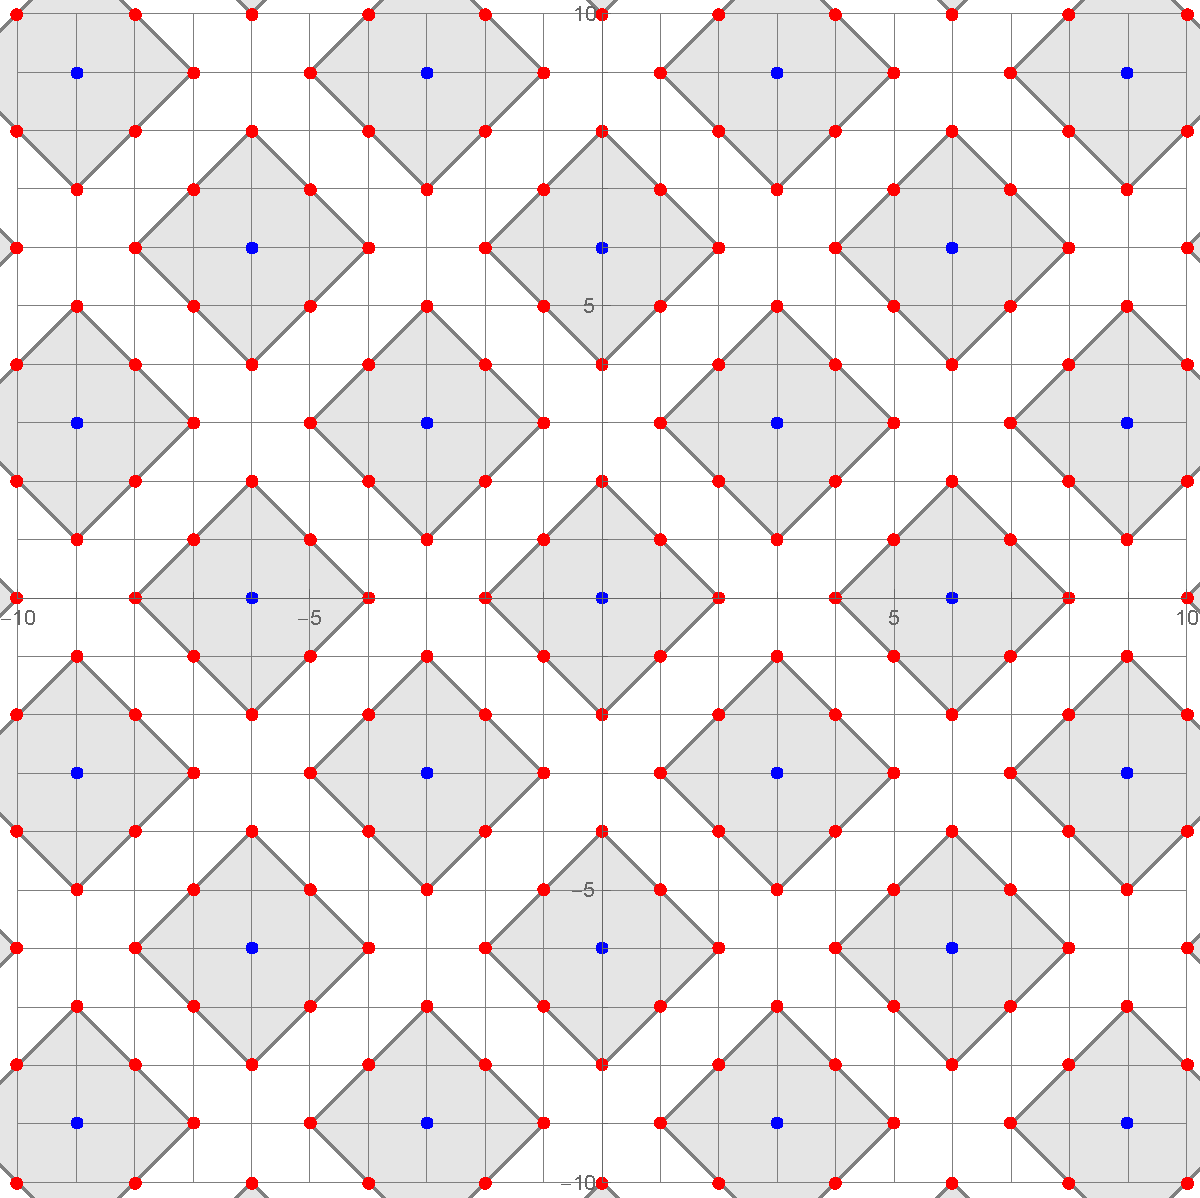
\includegraphics[scale=0.23]{exampler2l1.pdf} \label{fig1}
    \caption{Reticulado $\Lambda_1$ em $D_2$ na métrica $\ell_1$.}
  \end{figure}
\end{example}

\begin{observation}
  O reticulado $\Lambda_1$ também é um $r$-código linear perfeito em $D_2$ na métrica $\ell_2$.
\end{observation}

\begin{figure}[h!]\label{fig2}
  \centering
  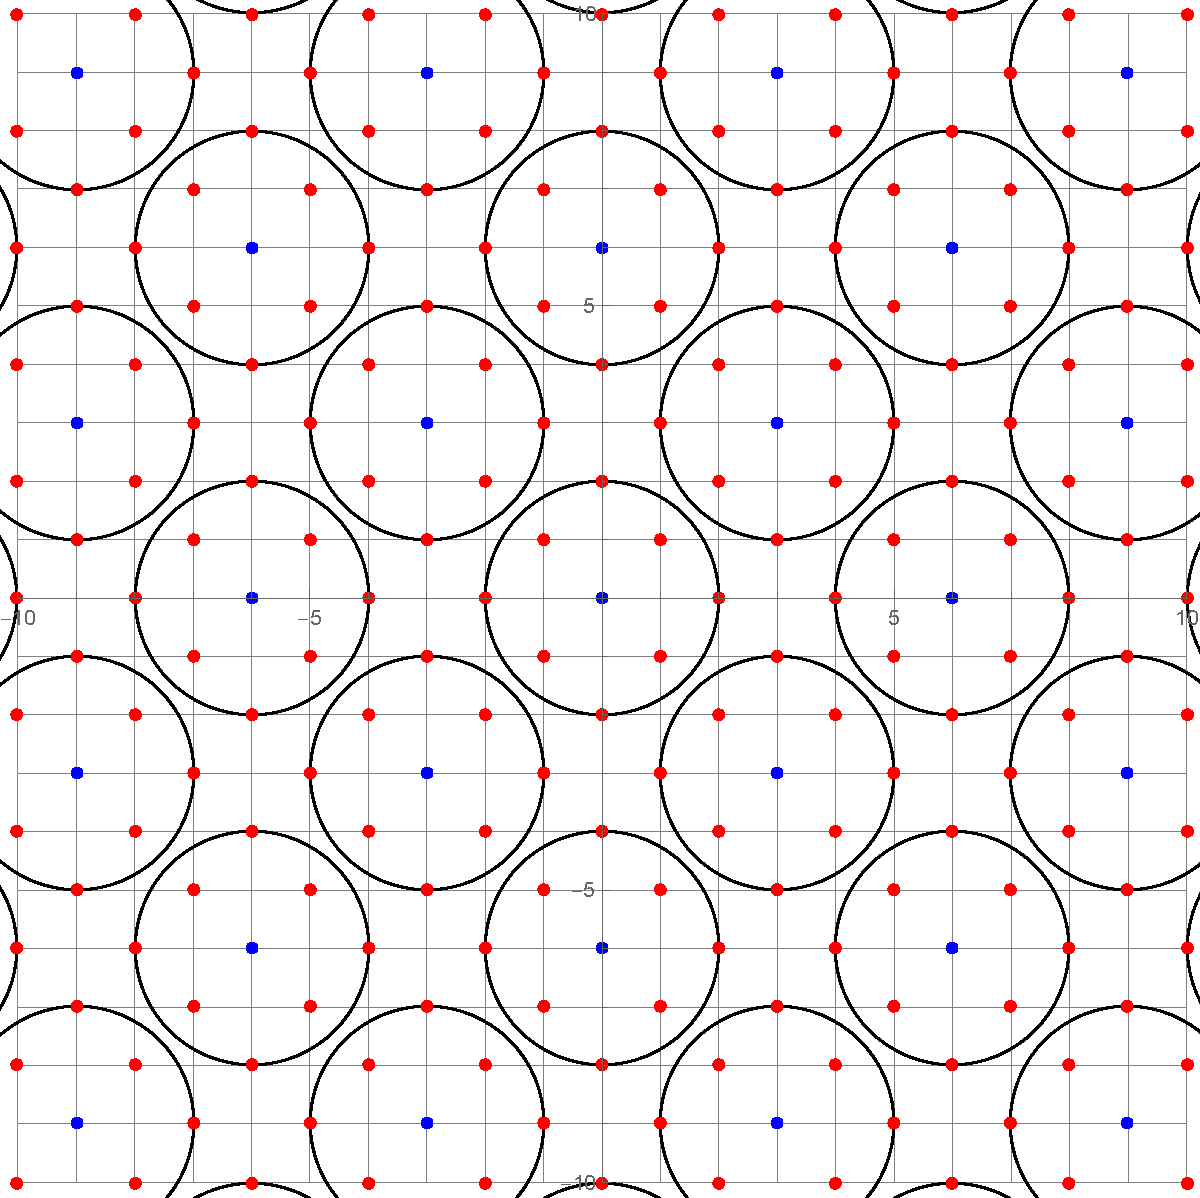
\includegraphics[scale=0.23]{exampler2l2.pdf}
  \caption{Reticulado $\Lambda_1$ em $D_2$ na métrica $\ell_2$.}
\end{figure}

\begin{example}
  Tomemos agora $r=4$. Pelo Teorema , temos que o reticulado $\Lambda_2$, com base $\beta_2=\{(0,10),(5,5)\}$ é um $4$-código linear perfeito em $D_2$ na métrica $\ell_1$, como pode ser visto na Figura. Além disso, temos que $\Lambda_2$ também é um $4$-código linear perfeito em $D_2$ na métrica $\ell_2$.
  \begin{figure}[!ht]
    \centering
    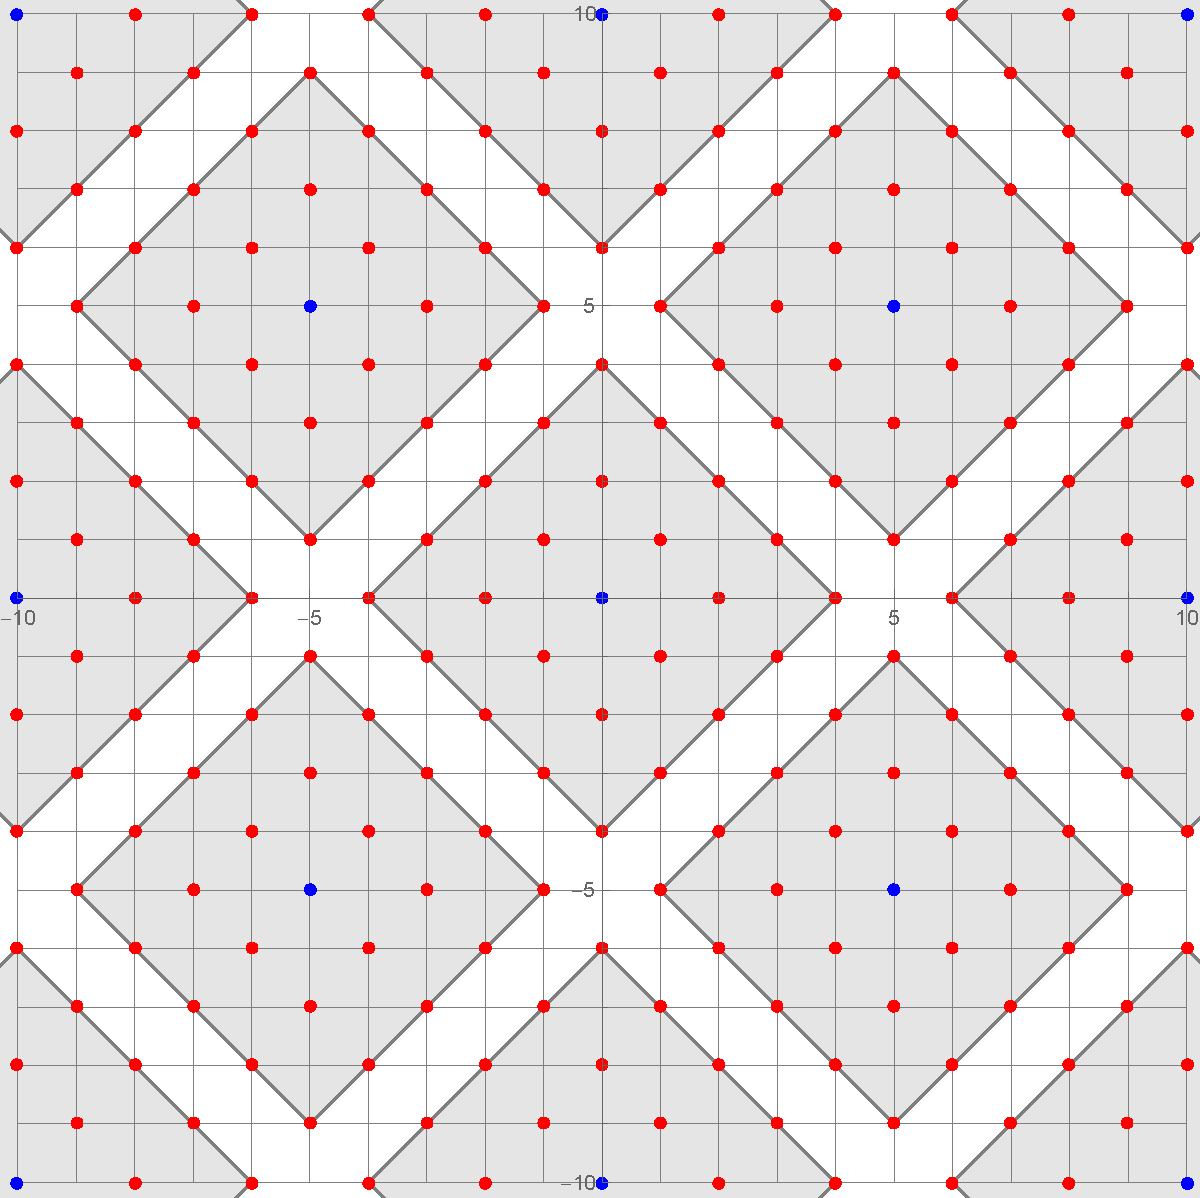
\includegraphics[scale=0.23]{exampler4l1.pdf}\;\;\;\;\;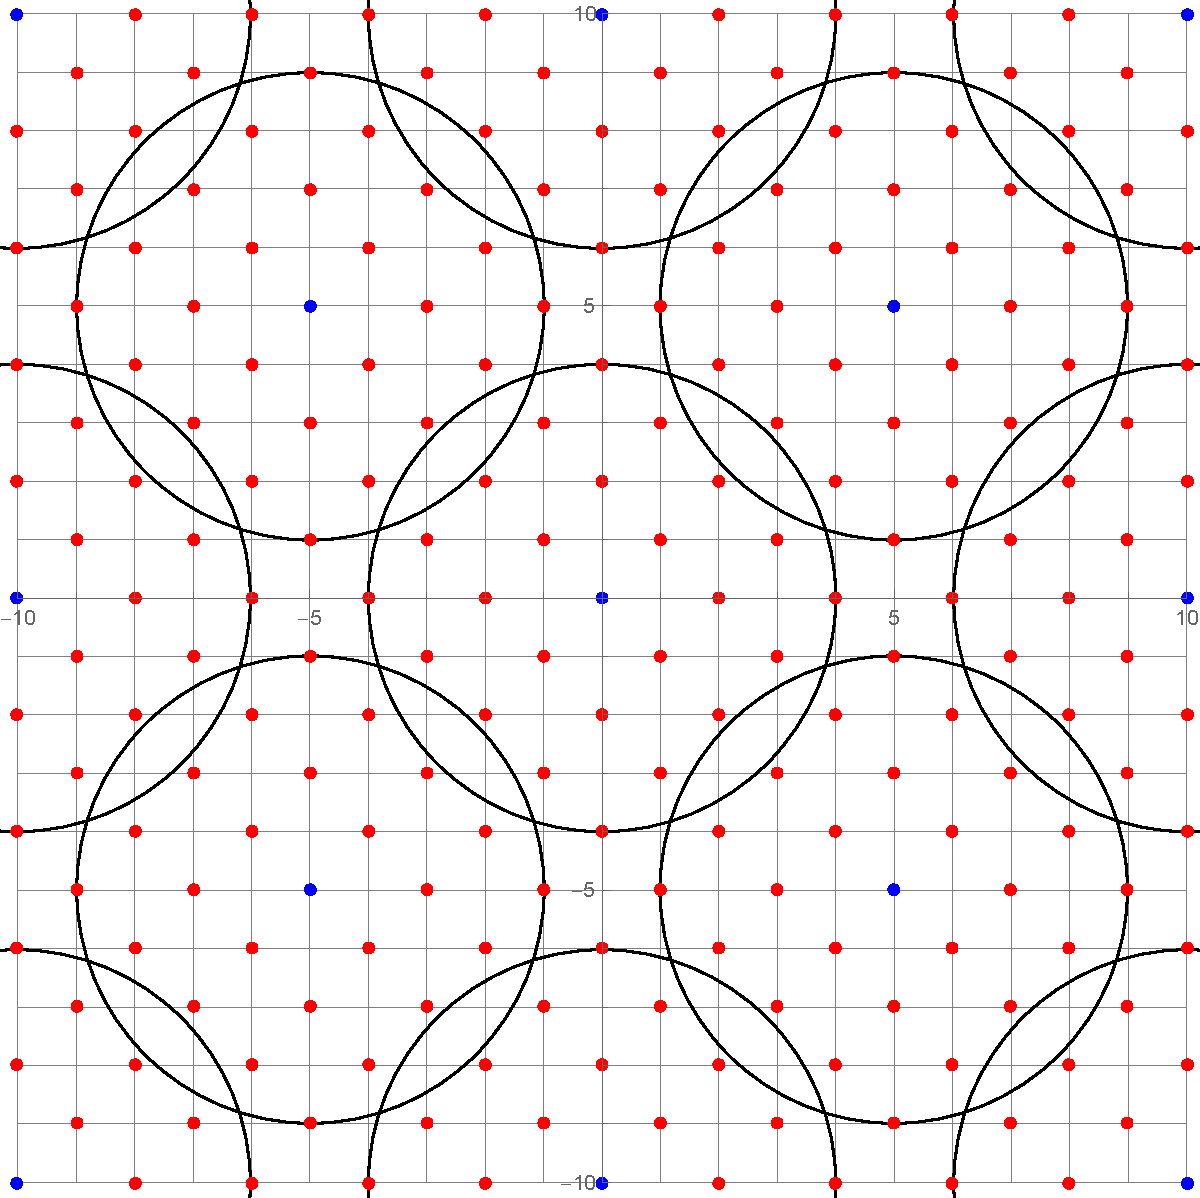
\includegraphics[scale=0.23]{exampler4l2.pdf}
    \caption{Reticulado $\Lambda_1$ em $D_2$ nas métricas $\ell_1$ e $\ell_2$ respectivamente.}
  \end{figure}
\end{example}

Notemos que, o reticulado simétrico de $\Lambda'$, obtido pela transformação linear $T: \mathbb{R}^2 \to \mathbb{R}^2$ dada por $T(x,y) = (y,x)$, é igual a $\Lambda'$. Isto é, $T(\Lambda') = \Lambda'$. Isso se da pelo fato de que $\beta''=\{(2(r+1),0),(r+1,r+1)\}$ é uma base para $T(\Lambda')$. Como $(2(r+1),0) = 2(r+1,r+1)-(0,2(r+1))$, isto é, pode ser escrito como combinação linear inteira dos elementos de $\beta'$, temos que os dois reticulados coincidem, já que $(r+1,r+1)$ pertence as duas bases.

Em $D_2$, consideremos os reticulados $\Lambda_3$ e $\Lambda_4$ com bases $\beta_3 = \{(5,1),(2,4)\}$ e $\beta_4 = \{(9,1),(4,6)\}$. Note que as Figuras e nos mostram que $\Lambda_3$ e $\Lambda_4$ são um $2$-código linear perfeito e um $4$-código linear perfeito respectivamente em $D_2$, tanto na métrica $\ell_1$, quanto na métrica $\ell_2$.

\begin{figure}[!ht]
  \centering
  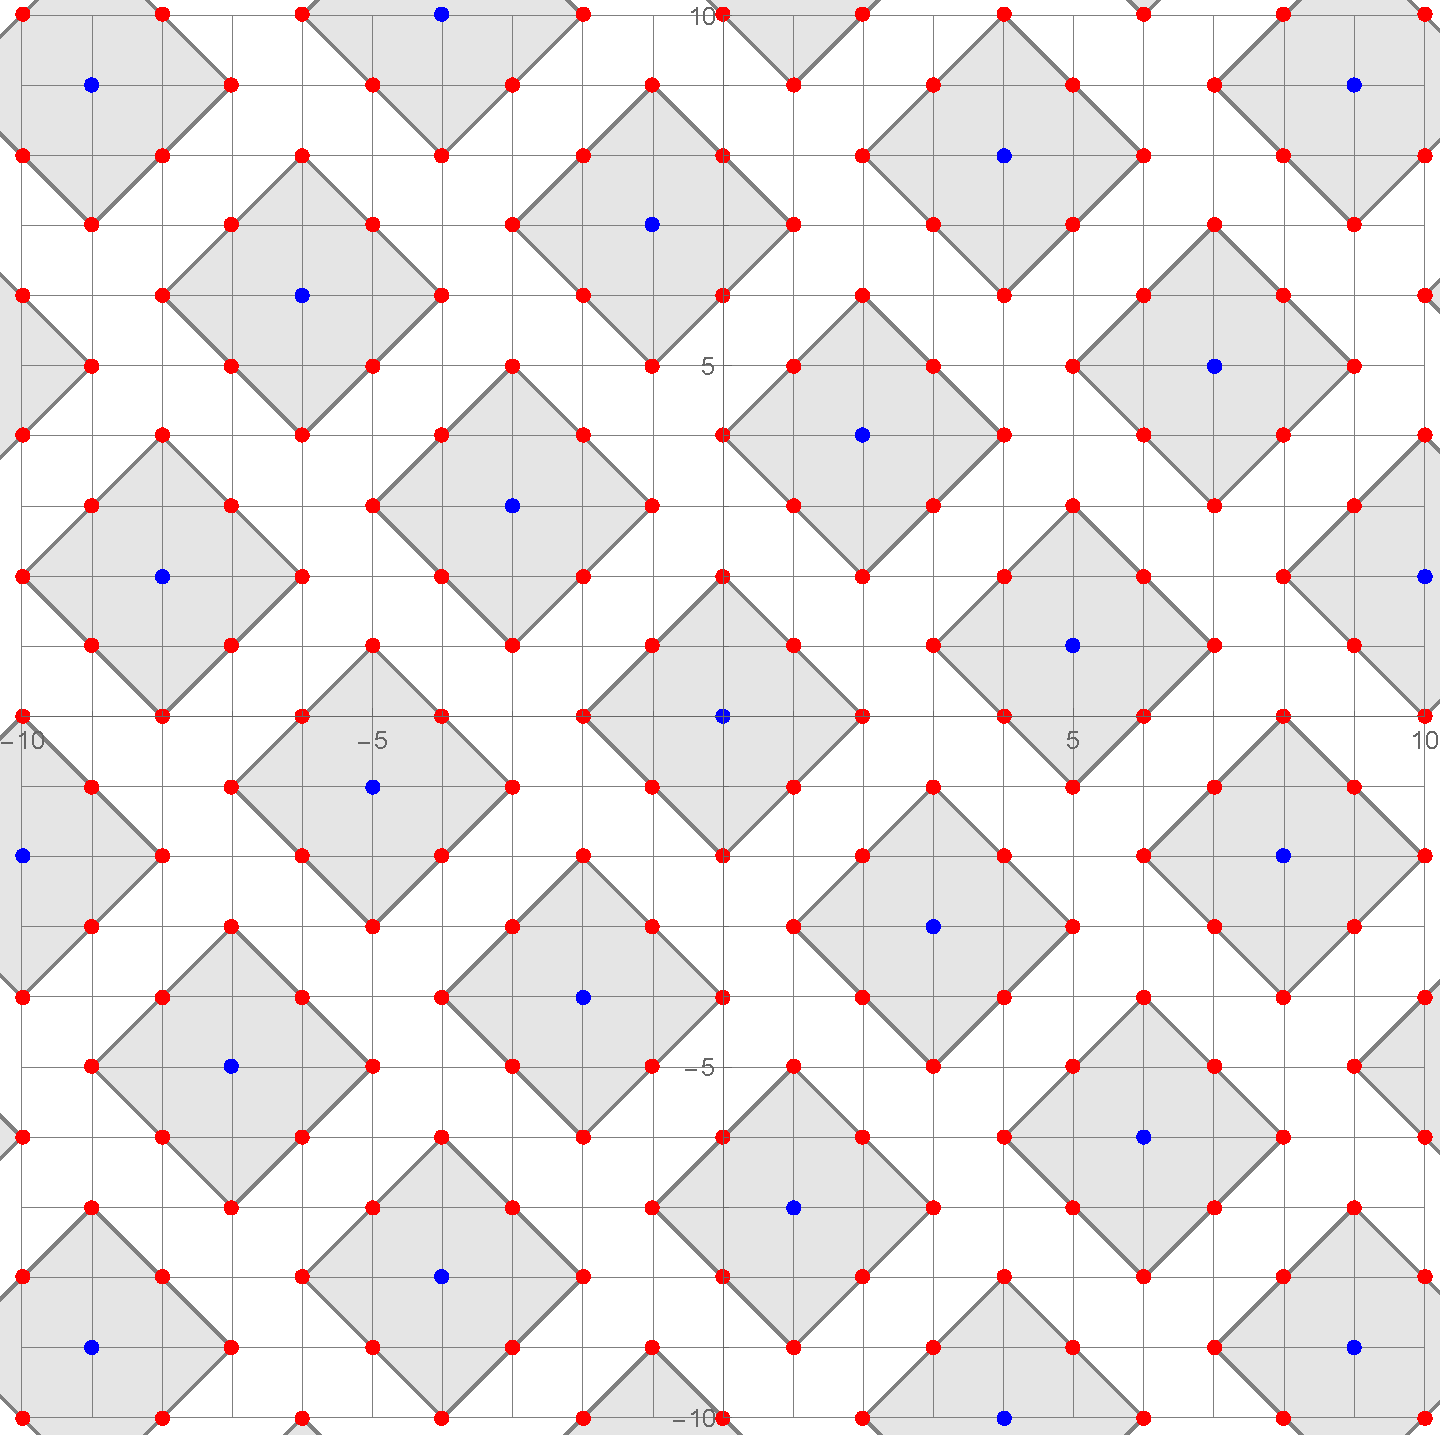
\includegraphics[scale=0.2]{newcoder2l1.pdf}\;\;\;\;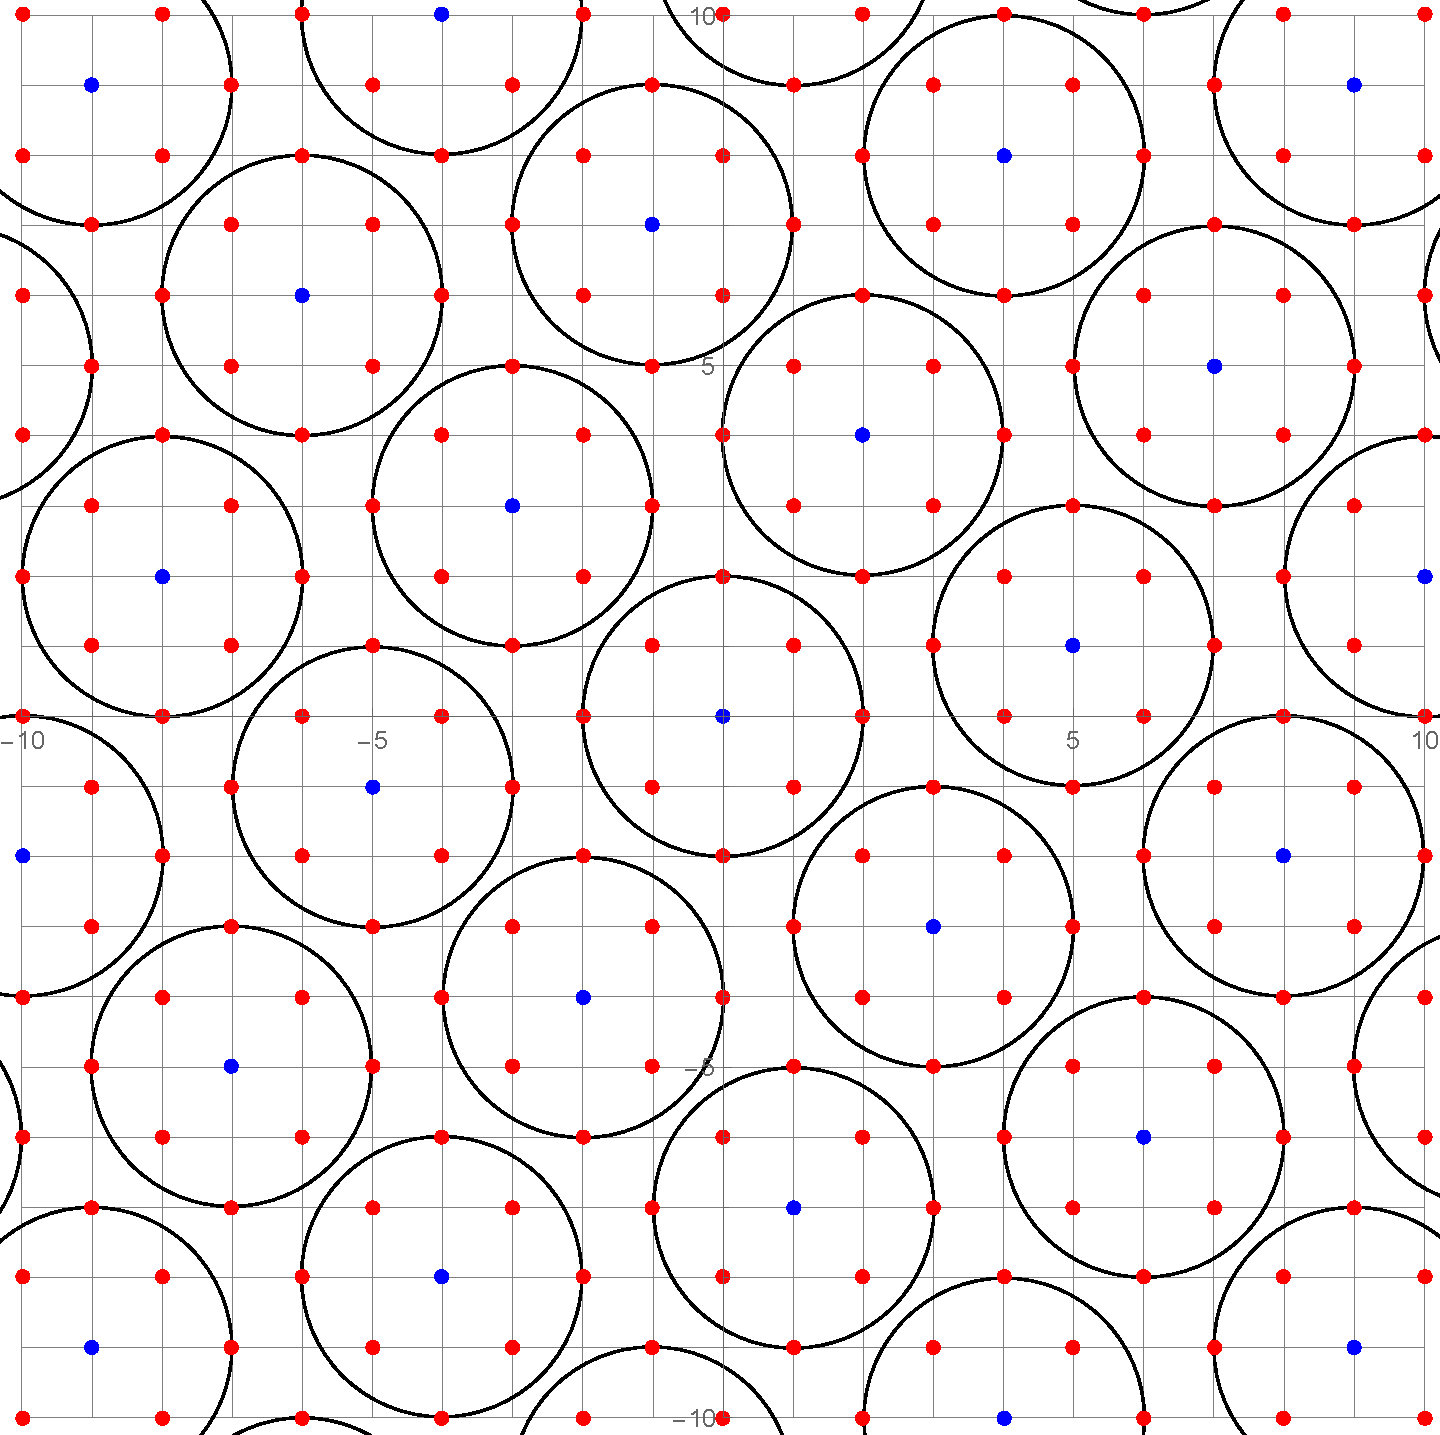
\includegraphics[scale=0.2]{newcoder2l2.pdf}
  \caption{Reticulado $\Lambda_3$ em $D_2$ nas métricas $\ell_1$ e $\ell_2$ respectivamente.}
\end{figure}

\begin{figure}[!ht]
  \centering
  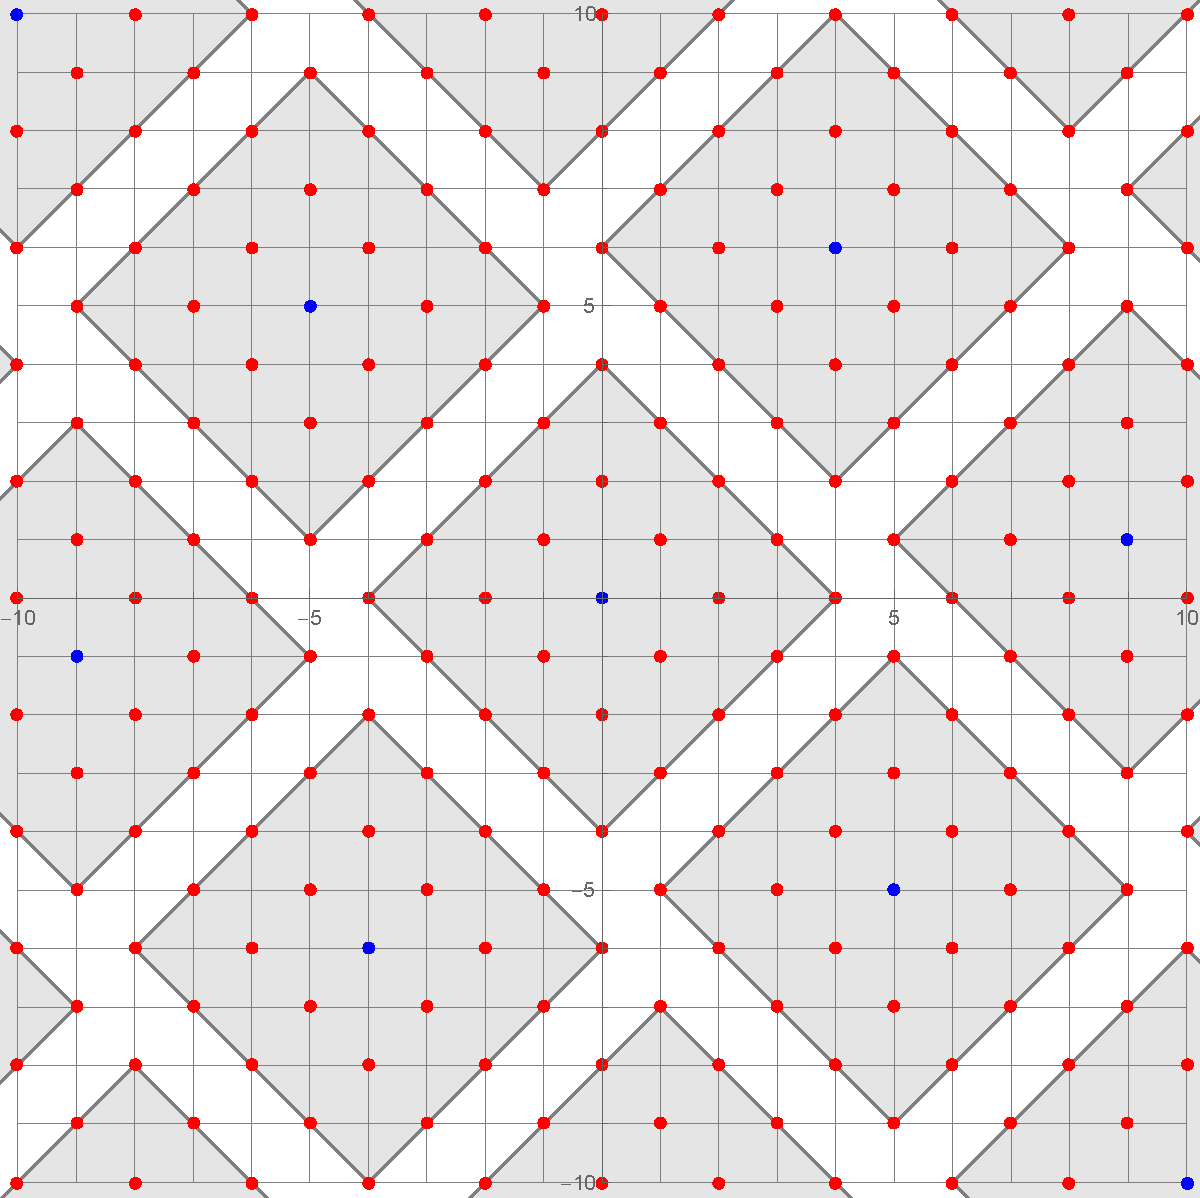
\includegraphics[scale=0.24]{newcoder4l1.pdf}\;\;\;\;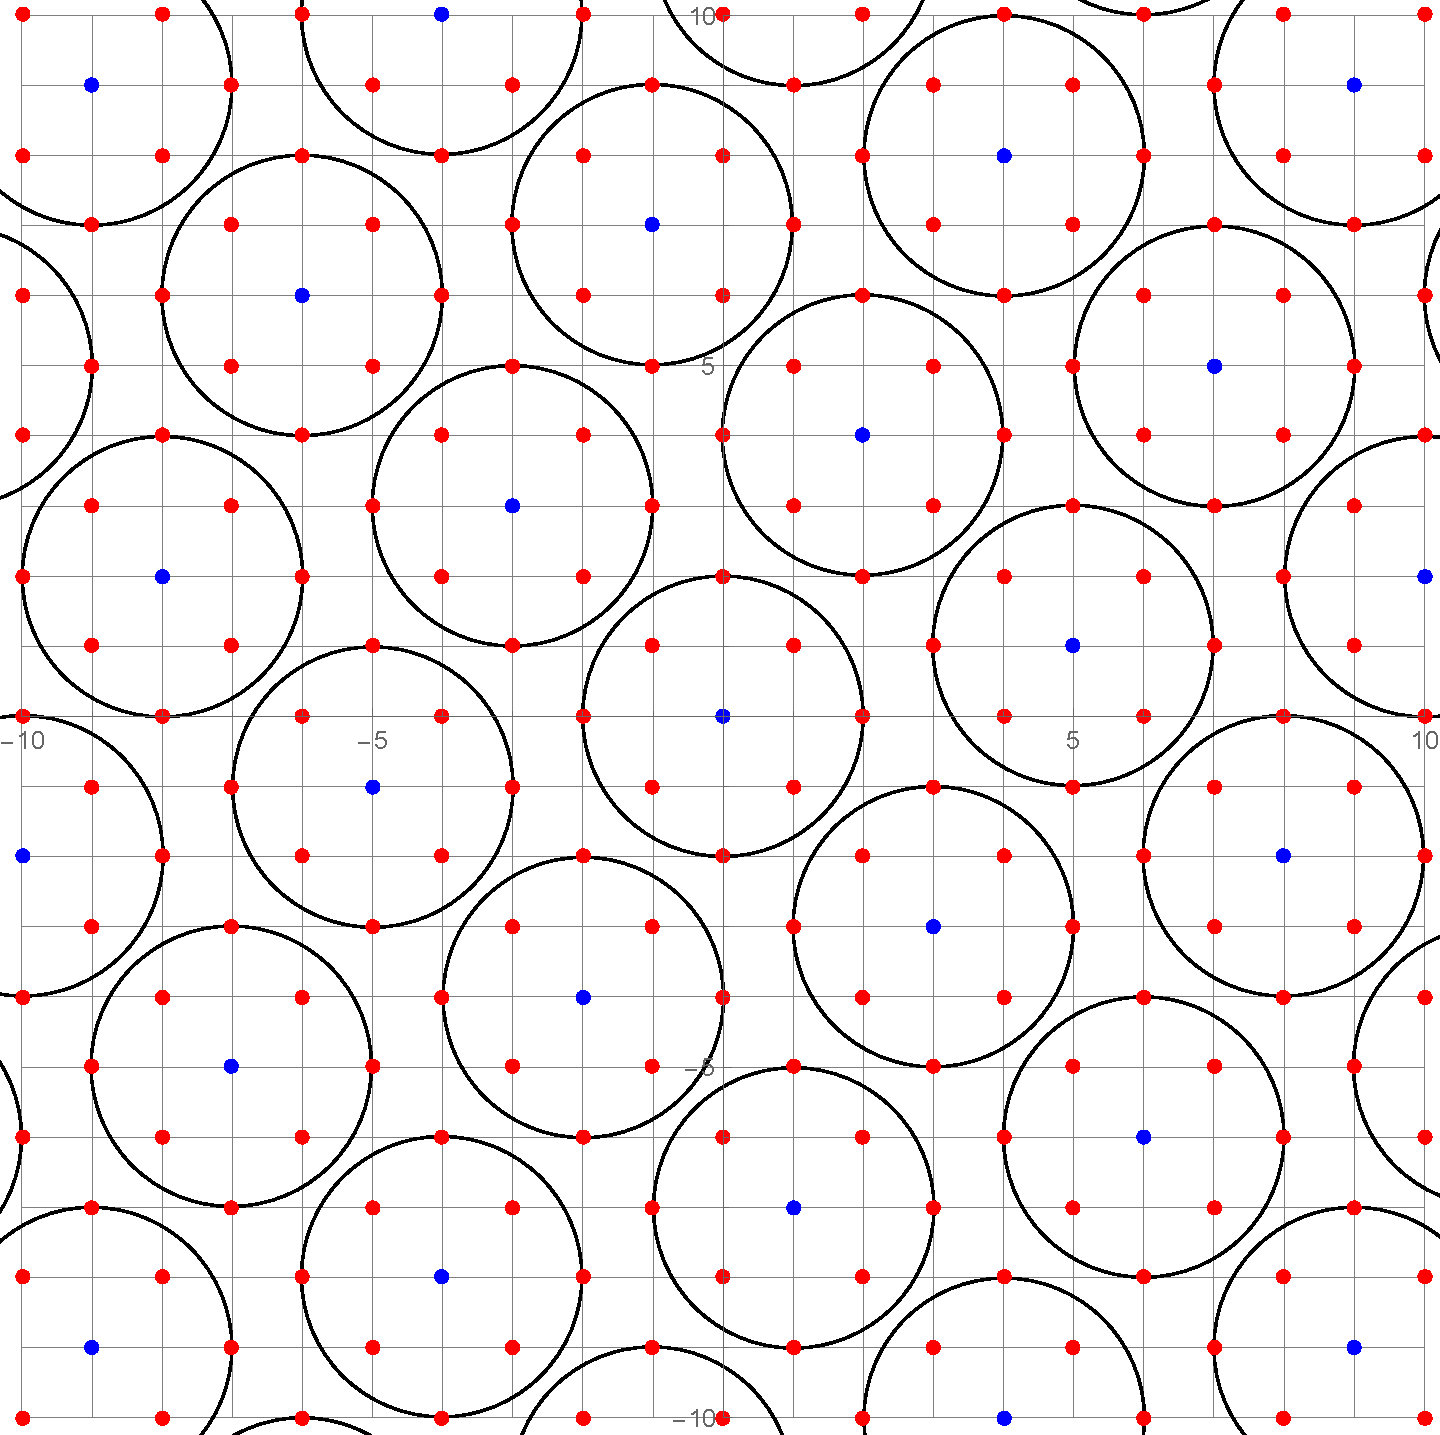
\includegraphics[scale=0.2]{newcoder2l2.pdf}
  \caption{Reticulado $\Lambda_4$ em $D_2$ nas métricas $\ell_1$ e $\ell_2$ respectivamente.}
\end{figure}

\begin{theorem}\label{cods2}
  Seja $r>0$ um número natural de modo que $r \equiv 0\;(\modu\;2)$. Temos que o reticulado $\Lambda''$, com base $\beta'' = \{(2r+1,1),(r,r+2)\}$ é um $r$-código linear perfeito em $D_2$ na métrica $\ell_1$.
\end{theorem}

\begin{example}
  Tomemos $r=6$. Pelo Teorema \ref{cods2}, temos que o reticulado $\Lambda_5$, com base $\beta_1=\{(13,1),(6,8)\}$ é um $6$-código linear perfeito em $D_2$ na métrica $\ell_1$.
  \begin{figure}[ht]
    \centering
    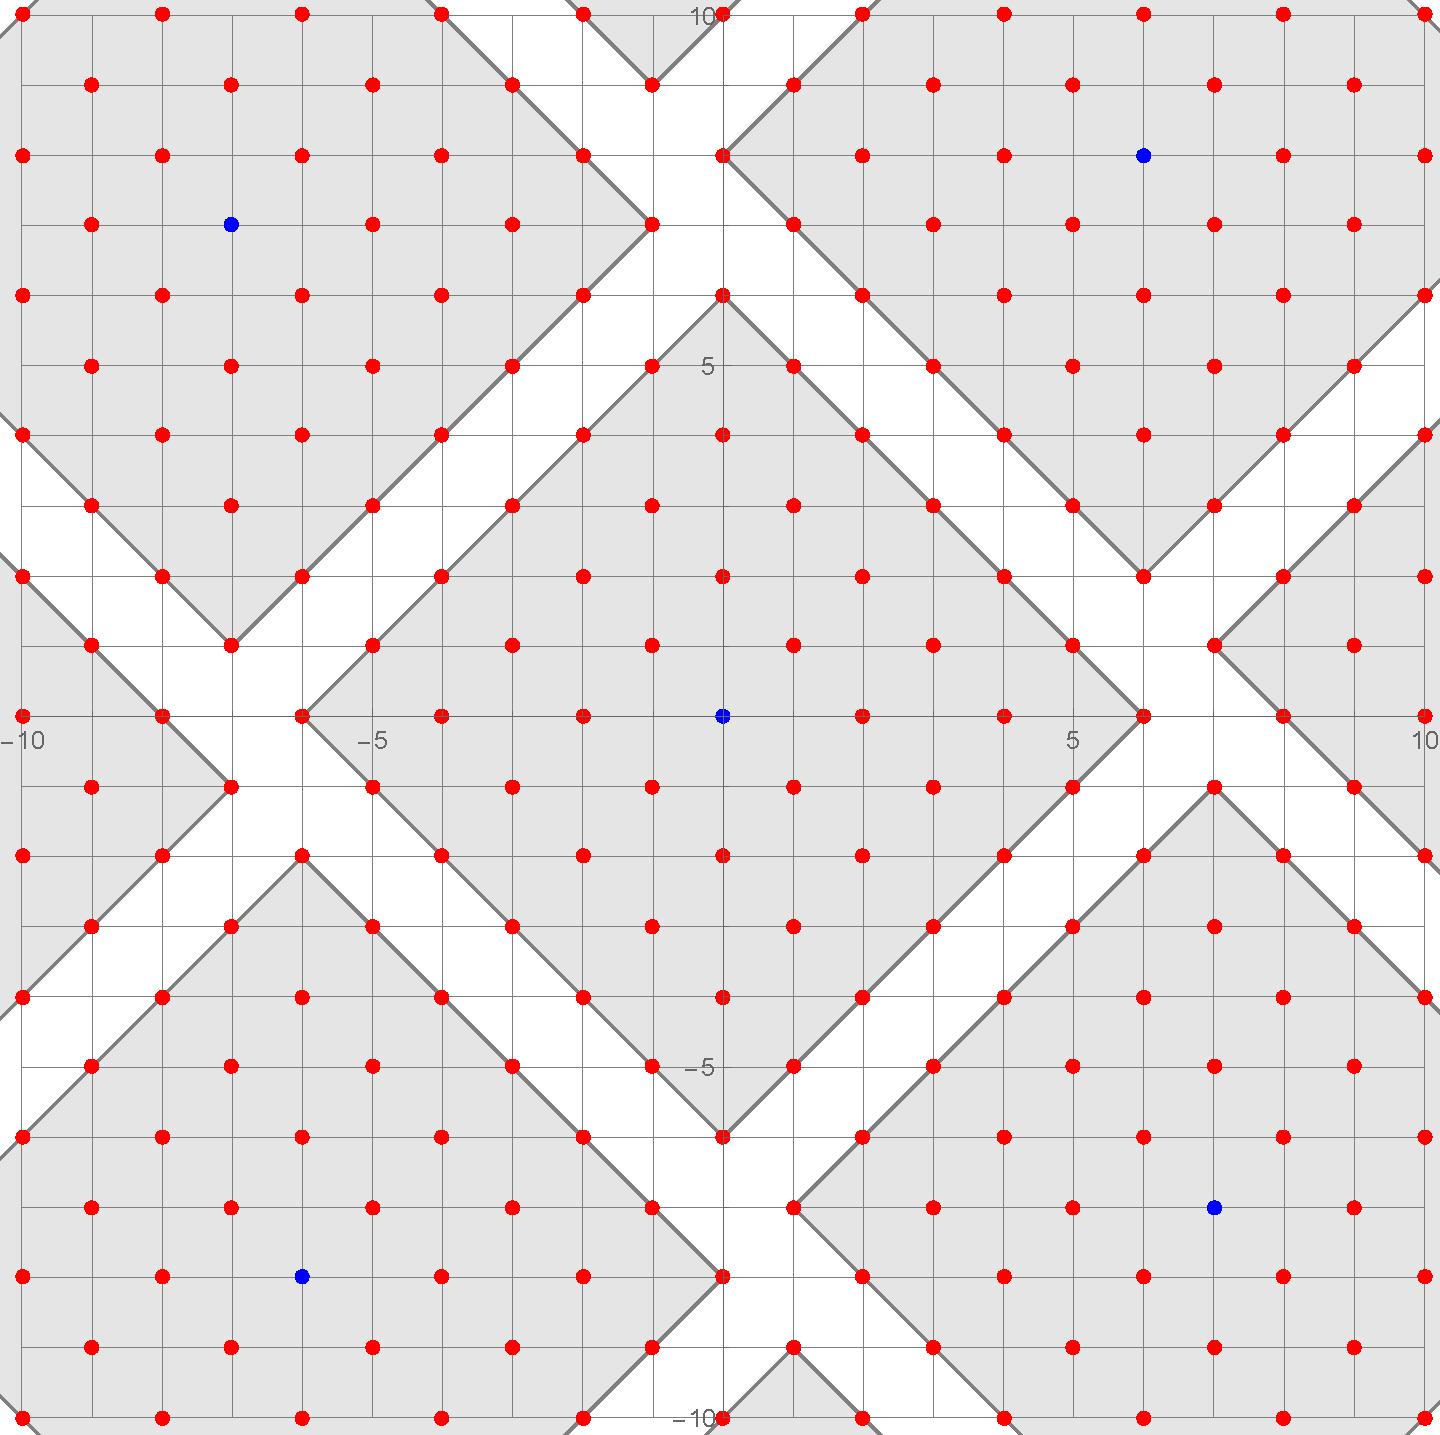
\includegraphics[scale=0.2]{code2r6l1.pdf}\;\;\;\;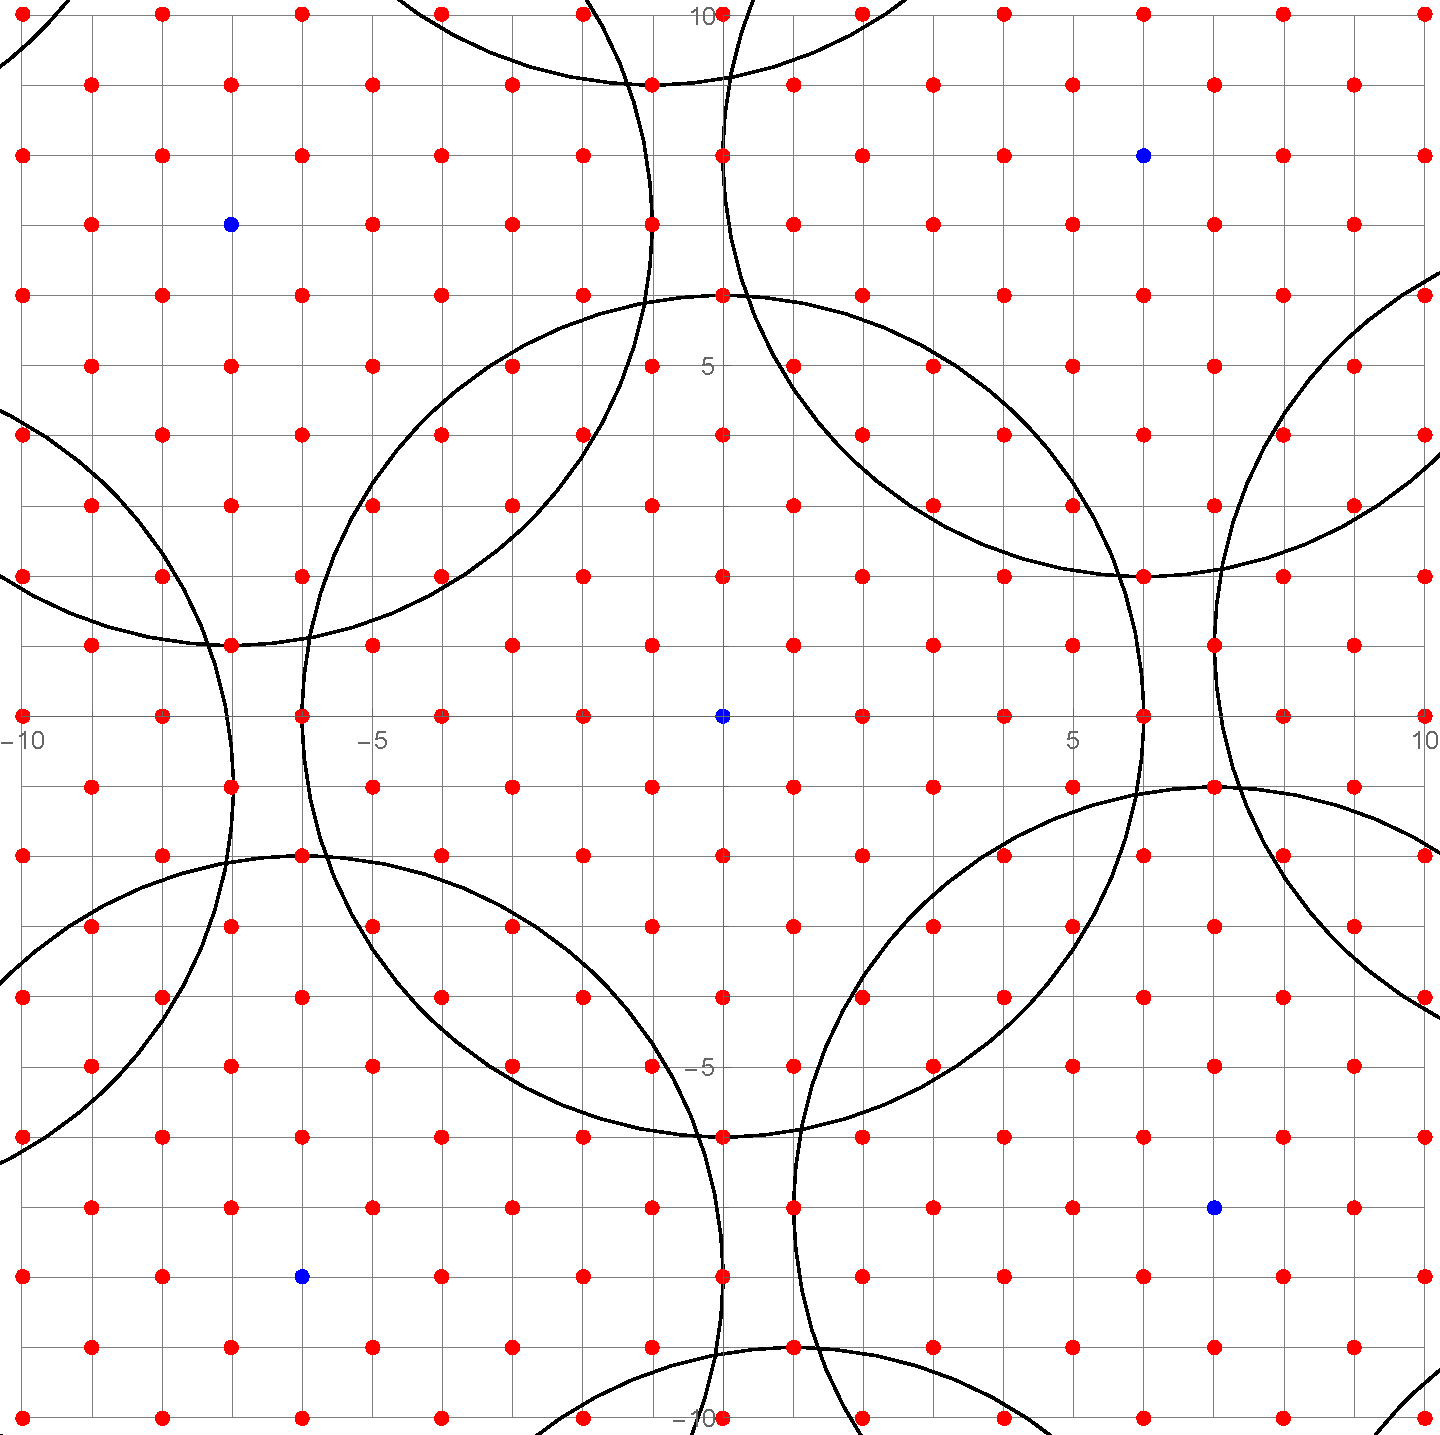
\includegraphics[scale=0.2]{code2r6l2.pdf}
    \caption{Reticulado $\Lambda_5$ em $D_2$ nas métricas $\ell_1$ e $\ell_2$ respectivamente.}
  \end{figure}
\end{example}

\begin{observation}
  Ao contrário do que aconteceu com $r=2$ e $r=4$, temos que $\Lambda_5$ não é um $6$-código linear perfeito em $D_2$. Uma vez que ao centrarmos bolas nos pontos de $\Lambda_2$, podemos ver que suas intersecções não são vazias em $D_2$, como segue na Figura 6.
  \vspace{0.5cm}
\end{observation}

De modo análogo ao o que ocorreu com o reticulado $\Lambda'$, temos que o simétrico do reticulado $\Lambda''$ também é um $r$-código linear perfeito em $D_2$ na métrica $\ell_1$. Isto é $T(\Lambda'')$  um $r$-código linear perfeito em $D_2$ na métrica $\ell_1$, como segue na Figura 7, tendo como exemplo o reticulado simétrico de $\Lambda_3$.

\begin{figure}[ht]
  \centering
  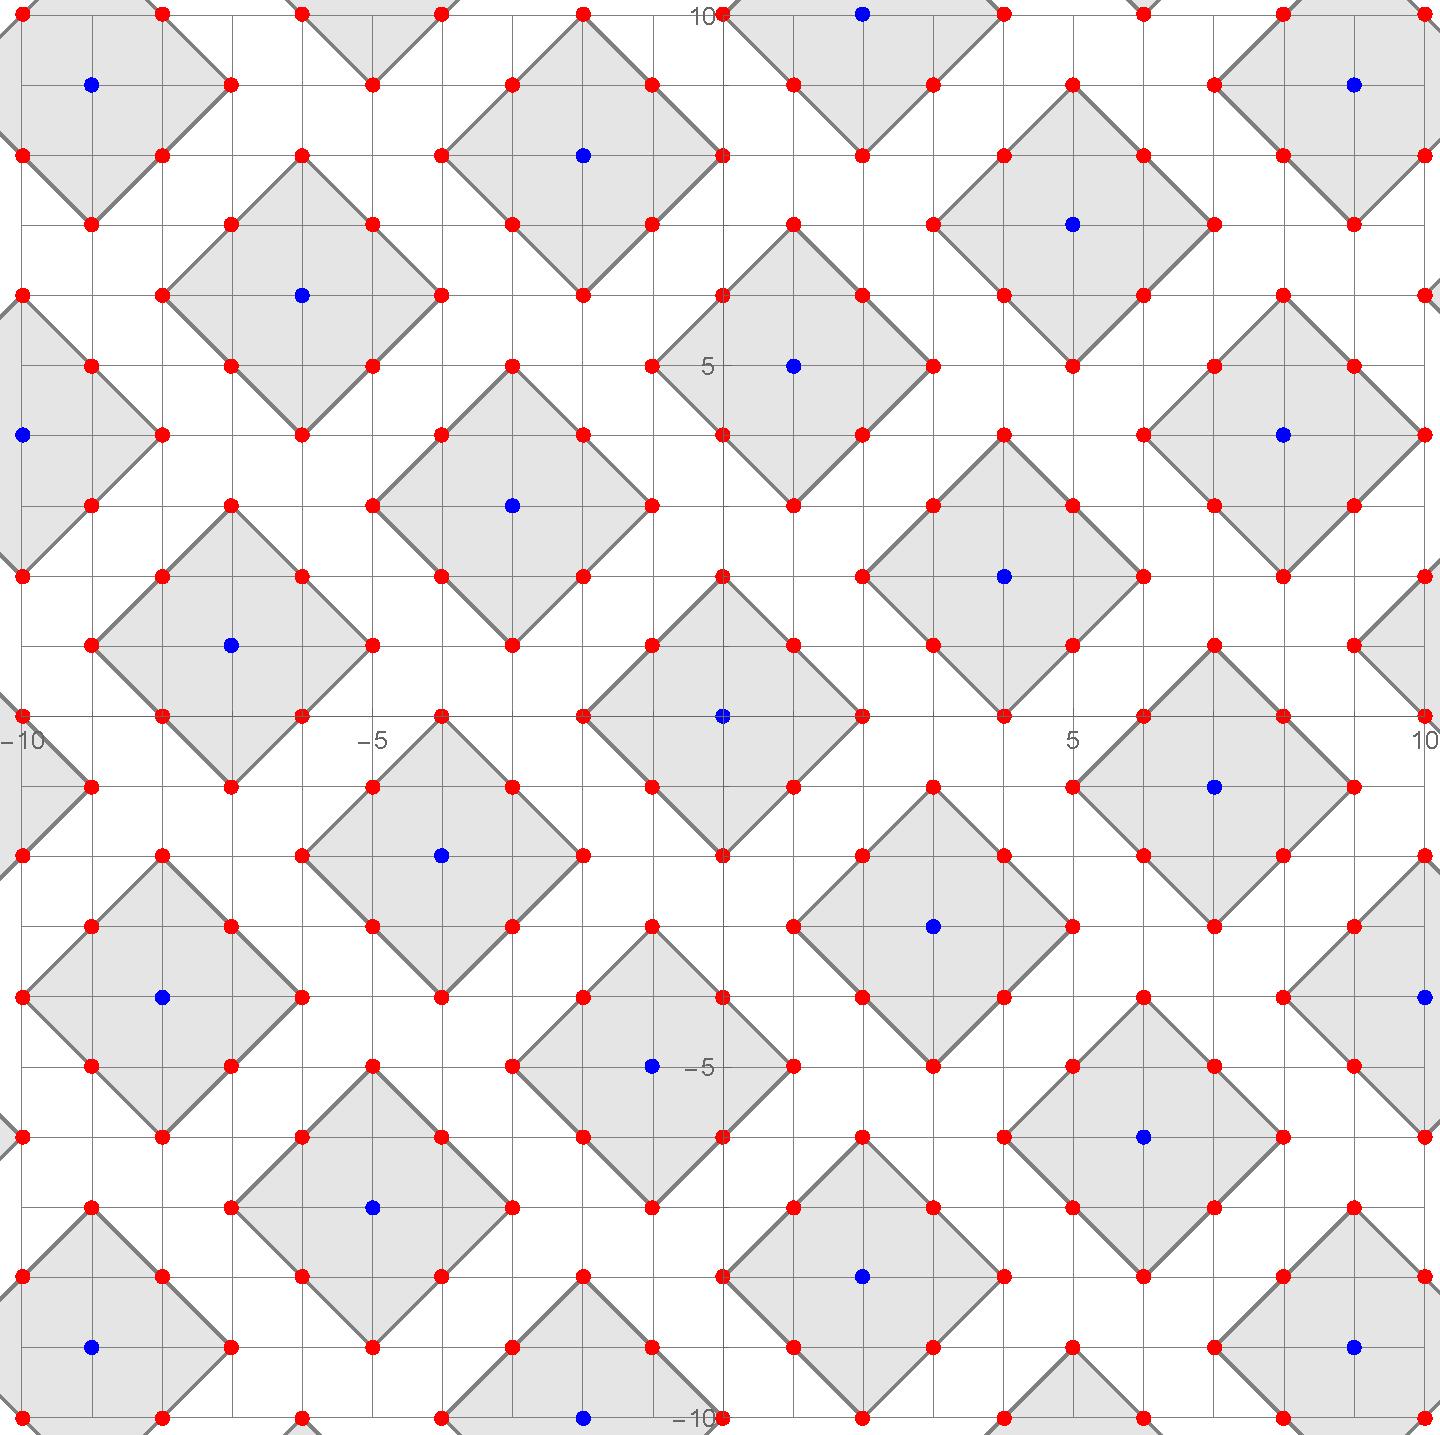
\includegraphics[scale=0.23]{simr2l2.pdf}
  \caption{Reticulado $T(\Lambda_3)$ em $D_2$ na métrica $\ell_1$.}
\end{figure}

Note que tanto no Teorema \ref{cods1}, quanto no Teorema \refeq{cods2}, temos que a distância entre os elementos da base de todos esses códigos são é dado por $2(r+1)$, mais ainda, a diferença entre cada coordenada é $r+1$. Mas isso não implica que todo reticulado que satisfaça essa propriedade é um $r$-código linear perfeito em $D_2$ na métrica $\ell_1$. Tomemos $\Lambda_6$ o reticulado que possui a base $\beta_6 = \{(6,4),(3,7)\}$. Note que a distância entre $(6,3)$ e $(3,7)$ é dada por $2(2+1)$ e cada coordenada difere $(2+1)$. Porém pela Figura 8 é fácil perceber que $\Lambda_6$ não é um $r-$código perfeito linear em $D_2$ na métrica $\ell_1$.

\begin{figure}[ht]
  \centering
  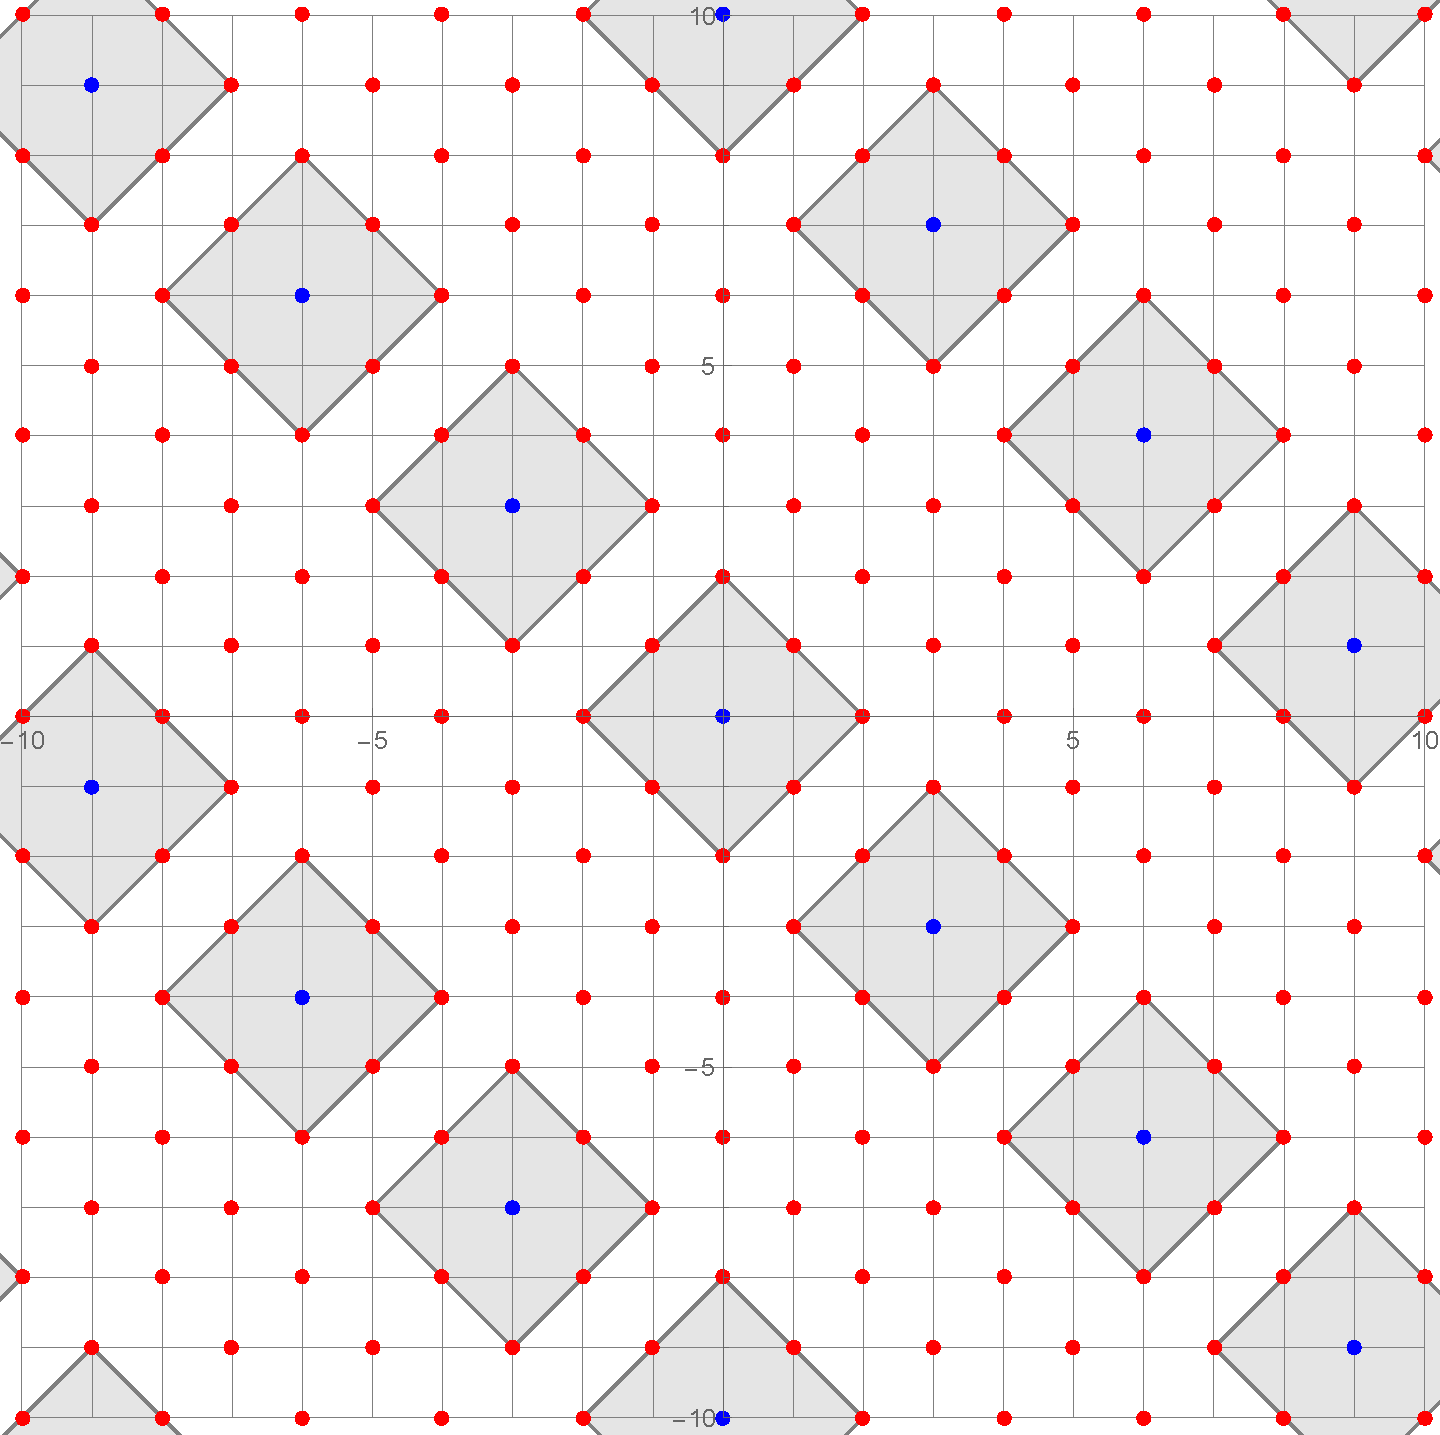
\includegraphics[scale=0.23]{notperfect.pdf}
  \caption{Reticulado $\Lambda_6$ em $D_2$ na métrica $\ell_1$.}
\end{figure}

\hspace{-0.5cm}\textbf{Pergunta:} Sabemos que isometrias em reticulados são dadas por composição de operadores ortogonais e translações. Além disso, sabemos também que se dois reticulados $\Lambda'$ e $\Lambda''$ são isométricos, então possuem a mesma densidade de empacotamento. Se $\Lambda'$ e $\Lambda''$ são congruentes, isto é, equivalentes com fator de dilatação $\lambda=1$, e $\Lambda'$ é um $r$-código perfeito linear em um ambiente $\Lambda_a$, temos necessariamente que $\Lambda''$ é um $r$-código perfeito linear em $\Lambda_a$?

\end{document}
